\documentclass{scrartcl} 
\usepackage{natbib}
\usepackage[T1]{fontenc}
\usepackage{graphicx}

\begin{document}  
\title {Summary of Findings of Supervised Research}
\subtitle {Consideration of distributed and parallel contour tree construction methods with task parallel paradigm in mind}
\author {Kilian Werner}
\pagenumbering{Roman}
\maketitle
\begin{abstract}
In this research documentation a method for construction of an augmented contour tree with a hybrid (distributed and parallel), task-parallel scenario in mind will be explained. Concurrent approaches to parallel contour tree construction will be reviewed, the most fitting method will then be adjusted and extended to our scenario. We will also explore topological simplification and especially our options to perform that on the fly during the computation of the contour tree, because this task fits well in our scenario. Lastly an effort was taken to tackle a truly parallel solution for merging split and join tree, but the results did not promise sufficient runtime benefits.
\end{abstract}
\newpage
\tableofcontents
\newpage
\pagenumbering{arabic}
\section{Exploring concurrent methods}  % This command makes a subsection title.

A considerable amount of work in this research consisted of exploring concurrent methods for parallel and/or distributed construction of contour trees and choosing one to adapt for the hybrid, task-parallel augmented scenario.

The efforts to find a method for parallel and/or distributed construction of contour trees are of a manageable amount. As follows is a list of methods and reasons each why an adaption to our context was not feasible.

\paragraph{The first approach} to a parallel contour tree computation was done by Pascucci et al. \cite{pascucci1} Their approach is simple, yet still feasible: First, the mesh is divided into chunks of almost equal size. Second, the split/join tree is computed for each chunk in parallel, but sequentially within the chunks in the classic ordered traversal union-find manner. Third, the local join/split trees are composited hierarchically. Each composition is sequential in nature and due to the reduction like communication pattern, there will be idle capacities in the later composition rounds. Finally the gathered join and split tree are merged to form the contour tree in a sequential matter.

While this approach may be adjusted to distributed memory scenarios, the top heavy, hierarchical nature implies a lot of global barriers, large portions of the code are still sequential and there is only one way to adjust granularity, namely by shrinking the size of the chunks, which will also increase the surface area between the trees that need compositing. This approach also does not compute an augmented contour tree by nature. Keeping track of augmentations while compositing trees may result in extraordinary overheads in a distributed context.

\paragraph{Maximum lists and path lists}
A different approach is taken by Maadasamy et al. \cite{Maadasamy}. Here the data is iterated over in arbitrary order (and possibly in parallel) finding all critical points and monotone paths from each critical point that is no extremum (so from each saddle) to extrema. This results in a maximum list storing all maxima that are reached by a certain critical point and a path list storing all critical points whose paths terminate at a certain maximum. These two lists will then be used to construct the join/split tree in a sequential manner, after which the two of them are merged to form the contour tree in a sequential manner.
This approach has a shared memory in mind and will require a global gather of the two lists and a barrier before continuing with the then local construction of the trees. Since not every vertex is traversed to form the two lists, obtaining an augmentation of the vertices is not inherent to this method.

\paragraph{Distributed Contour Trees}
A recent approach by Morozov et al. \cite{Morozov} is aimed towards a distributed setting and computes a distributed representation of the contour tree, by observing that every vertex lies on exactly one path between a local minimum and local maximum. This approach is in itself quite feasible and would not need adaption to our scenario, but inherently does not produce an actual augmented contour tree for general purpose use cases. While we cannot make use of this approach for that reason, its existence implies, that our goal includes to produce an actual contour tree on one single node, since another distributed representation seems unnecessary. 

\paragraph{Domain space subdivision}
Charles et al. \cite{Charles} take a somewhat different approach. Instead of subdividing the mesh in a spatial manner, they subdivide it using iso level sets. Now inside of each chunk a contour tree can be computed and all arcs that lie completely inside the level set of the chunk are already correct arcs in the contour tree. In a similar fashion to \cite{pascucci1} the local trees are now merged hierarchically until the contour tree is complete. This shares of course the disadvantages of top-heavy reduction like operations, but has the additional disadvantage, that for fine grained parallelism possibly a dominant amount of local arcs will need stitching over multiple iterations, especially arcs with high persistence. Also the subdivision along level sets needs to be computed first and for fine grained parallelism the actual number of vertices in a chunk may become smaller than the number of necessary ghost cells. Again the stitching process is sequential. However this method would yield an augmentation of the data quite easily. Note that this approach is the only approach that does not need a sequential merge of the global split and join trees in the end.

\paragraph{Peak Pruning}
Carr et al. \cite{Carr} explore an approach fitted for SMP. From each vertex a monotone path walks to an extremum. W.l.o.g. let's talk about maxima (split tree). Saddle candidates for maxima are then vertices whose ascending neighbors walks contain at least two different maxima. Among these saddle candidates the highest value is chosen to be the actual saddle of the maximum which adds an arc to the tree. The maximum is then pruned to the saddle and a recursive strategy finds further arcs. This approach is very feasible and the notion of saddle candidates that can possibly walk to multiple extrema and actual saddles that are the most extreme saddle candidate for an extremum will be found in our solution too. However for a distributed memory scenario with far less possible threads than vertices in the data we will be taking a somewhat reversed approach: Walking from the extrema and not to them. This is to minimize messages between neighboring chunks of data and is also a more straightforward approach when not in an SMP environment. 

\paragraph{Sweep to Saddle}
Lastly another approach is found in the field of ad-hoc networks. Sarkar et al. \cite{adhoc} explore the possibility to make an ad-hoc network of sensors aware of their contour tree. Each local maximum starts a sweep, which carries the id of the maximum. The sweep can continue in parallel to every vertex whose more extreme neighbors have also been swept with the same id. This sweep will eventually terminate and therefore identify a boundary of unsweepable vertices. Those can only be unsweepable, because they have more extreme neighbors that cannot be reached by the sweeping extremum, because they belong to a different extremum. Therefore in great similarity to \cite{Carr} we found the saddle candidates and need only choose the most extreme of them to form an arc of the join/split tree. Once a saddle was found in that way by all it's maxima it can continue the sweeps of them at their boundary recursively.

This last approach is the main inspiration for our solution. It was adapted to a hybrid, HPC and task-parallel scenario and extended to compute the augmentation as well. Our final solution is therefore somewhere between \cite{Carr} and \cite{adhoc}.

\section{A join/split tree construction method with task parallelization and AGAS distribution in mind}

\subsection{Approach, Idea and Theory}

\paragraph{Subdivision}
Most of the introduced approaches achieve parallelization through subdividing the data set either spatially or in the reeb function domain. In a distributed HPC environment the data is typically too large to be stored in a single nodes memory, so this subdividing will be present in our approach too. However such subdividing on its own usually does not inherently yield the fine grained parallelization targeted by a task-parallel approach. Dividing the data in so many chunks, with only one, sequential subtask per chunk, that these tasks can fill the work-queue, providing a high enough occupancy to allow for latency hiding and the likes, is not feasible; especially when reviewing the top-heavy stitching processes necessary to conquer, after this division. 

Therefore our approach will work with the data arbitrarily divided into one chunk per node and try to create fine grained local parallelism in each chunk, while also circumventing any additional computation to merge any partial solutions from the chunks. We will keep in mind, that it should still be possible to further subdivide chunks to allow for out-of-core and work-stealing extensions of the approach. 

This leads to the question: Given a fixed mesh (may it be the total mesh or a chunk of it), how could one create a parallelization with a proper grain for a multi-core system and a task based approach? This is where we adopt some observations made by \cite{Carr} and \cite{adhoc}. Note that w.l.o.g. we are talking about the join-tree, where local minima spawn new arcs. Generally for the split tree, "minima" has to be switched with "maxima" and "smaller" with "higher" function values.

\paragraph{Observation}
The join tree has exactly one arc, representing one connected level-set component, for every local minimum and every saddle point in the data. An arc in the join tree will only ever reach one merge node (or the global maximum in the end). Therefore the complete tree can be represented by a map, mapping critical points to their respective saddle / merge node. If we can identify all critical points and find their respective saddle / merge node in parallel, join tree construction will be solved. In the following a critical point will be taken to represent the arc that starts at it.

\paragraph{Finding local minima} can be easily done in parallel: Iterate over each vertex in the data (chunk) and check if its function value is less than the function values of all its neighbors. Since function values and neighboring information does not change this iteration can be parallelized in a thread safe manner by just assuring simultaneous reading is possible. Note that we will not have to check every neighbor of every vertex, since for each local minimum found we will schedule a task to compute its arc and augmentation and each vertex that already belongs to an arc can never be a local minimum. We will therefore skip most vertices after finding the first few minima. Thread safety is still easy to achieve, since the correctness of the algorithm does not depend on these skips and if we check a vertex that was just added to an arc in parallel no problems arise.

Critical points that are not local minima will be discovered along with the construction of the contour tree, since all of them are also saddles / merge nodes which we will have to find anyways. Similar to the peak pruning in \cite{Carr} the saddle of an arc that starts at another saddle can be found just like the saddle of arcs that start at local minima, once all child arcs are dealt with. The main question remains, how do we find the saddle, for an arc of a given critical point? Consider the following observations:

\paragraph{Finding saddles for critical points}
The saddle / merge node of an arc will always be a vertex that is connected through a monotone path with the critical point that represents the arc. The path has to be monotone, because otherwise a vertex on the path to the merge node would at some iso-value have belonged to a distinct level-set component than the representing critical point, which would indicate that those two components would have merged before reaching the iso-value of the saddle in question, disqualifying this saddle as the merge node of the arc. This monotone path condition along with morse theory allows for an interesting observation: All points that can be reached by monotone paths from two different minima will always be located on the common boundary of the ascending manifolds of the minima. In other words the saddle point of an arc starting at a local minimum will always be located on the boundary of the ascending manifold of that minimum. Even more so, each vertex on that boundary could merge the connected component started at the minimum with another component and would therefore be the saddle, if no other merge would have happened "sooner" (at a lower iso value). Therefore the vertex on the boundary of the ascending manifold of a minimum with the lowest function value is guaranteed to be the merge node for the arc started at that minimum. 

To find the boundary of the ascending manifold, we can perform a BFS (let's call it sweep) starting at the local minimum, with the following characteristics:
A vertex v can be visited if all it's smaller neighbors have been visited, this assures that all possible monotone paths through v start at the minimum and therefore v belongs to its ascending manifold. Once a vertex is visited it adds all its neighbors to the queue, with vertices already visited being skipped. If a vertex that is taken from the queue is not allowed to be visited (because it has unvisited neighbors with smaller function value than itself) it is marked as a possible boundary vertex, once a vertex is visited this mark is removed. After the sweep terminates, all vertices marked as boundary form the actual boundary of the ascending manifold and the smallest marked vertex is the merge node of the represented arc. 

For the found merge nodes a check is performed, if all other arcs that end here have finished with their sweep. That is easily done by checking if all neighbors of the saddle with a lower function value than him has been visited by some sweep. The merge node then starts its own sweep with the following adaptions: The remaining boundaries of all ascending manifolds of the child arcs of the merge node are added to the BFS queue before start of the sweep. Also vertices visited by one of the children of the merge node (or their children and so on) are viewed as visited by the sweep of the merge node itself. 

This peak pruning like recursion finds all merge nodes for each critical point and constructs the join tree as represented by the mapping from critical point to saddles. In the end the last critical point will observe an empty boundary, which means that the highest visited vertex of the sweep is the global maximum and trunk of the tree. 

\paragraph{Augmentation}
For the augmentation consider the following: If the BFS were altered to run on a priority queue, so that each vertex visited is the smallest vertex on the current boundary of the sweep, then the first visited node that can not be swept due to smaller unvisited neighbors has to be the saddle of the current arc. In this case the BFS could terminate early and pass the remaining queue on to the saddle's sweep. In this scenario exactly the vertices visited by the sweep will belong to the augmentation of the represented arc. Therefore the augmentation will exist after the computation of the tree in the form of the map from each vertex to the critical point that visited it with its sweep. 

However trying to sweep in an ordered manner will eliminate the possibility to parallelize the sweeps and leave us with a sequential sweep once we reach the trunk of the tree. Even worse, if a sweep crosses the boundary between data chunks in the distributed scenario, the two nodes will have to maintain a shared priority queue, eliminating parallelism and resulting in possibly huge amounts of messages. Therefore in our solution we will stick to the sweeps being done in arbitrary order, allowing a critical point to visit nodes, that do not belong to its branches augmentation. Luckily these prematurely collected vertices will always find the arc they belong to among the path from their (possibly wrong) initial arc to the global maximum, because this sequence of arcs will always represent the growing level set component containing the part initially started at the critical point that visited them. Therefore the augmentation can be calculated in a post-processing step like this: Iterate over all vertices and check if their function value is larger than the saddle of the arc they are augmented to. If so move them to the arc that is started at this saddle and repeat until you reach the arc that represents your component at your given iso-value. 

\subsection{Task parallel, AGAS distribution in mind}
Now that we understood the approach of constructing the tree as a map from critical points to their saddles, we should already have an instinct telling us, that this approach can be implemented in a parallel way. Let's explore how exactly this approach yields good task parallelism, fits well with an AGAS based distribution and where exactly it's limitations are.

As already mentioned local minimum detection can be done in parallel. More precisely we can subdivide the data (chunk) into as many parts as we have worker threads on the node and spawn one task to iterate over them each. Each of these tasks is set to interrupt itself in favor of a new spawned sweep-task every time it finds a local minimum. As mentioned above the sweeps will allow us to skip large portions of the data in our search for local minima, but every time a sweep-task is suspended due to some latency, the minimum searching task may resume their work and potentially find new local minima. 

We are however not limited to the number of currently observed arcs in our parallelism. We might spawn multiple tasks that run the same sweep, thread safeness will be easy to assure, since we only need a thread safe queue-like data structure, which is even allowed to pop elements in arbitrary order. Note that even popping the same element twice because of race conditions would not pose a problem, only loosing an element in the data structure due to race conditions would destroy correctness of the algorithm. Instead of spawning multiple tasks from the start, we could start additional tasks for current arcs on demand, whenever resources become idle. Whichever approach we take, we should make sure, that the trunk, as a typically very large, single arc that will usually remain for a long time after all other arcs are done, can be swept in parallel by all resources we have. Note that boundary marking and keeping track of the minimum boundary vertex will require some synchronization between tasks, however for large arcs (that may have impact on performance) the boundary to interior ratio of an ascending manifold will be quite small, especially in higher dimensions.

With sweeps we may encounter data chunk borders while sweeping. Here AGAS comes into play. A sweep is initiated and labeled by the local minimum, which for that purpose receives a global address. When trying to visit a ghost cell (allowing us to check for local minima without communication to neighboring chunks) we will instead issue a sub-sweep on the corresponding data chunk, still labeled with the global address of the minimum. Keeping track of boundary and minimum boundary vertex will be a locally organized duty, once the local queue is empty the observed boundary along with minimum boundary vertex will be reported back to the holder of the global address the sweep was labeled with. Re-entering a data chunk that already works on that sweep will just add the reported vertex to the queue of that sweep, they can be matched thanks to the globally unique label of the sweep. It would still be possible for two neighboring data chunks to send messages back and forth if a sweep moves along their common boundary back and forth very often. This can be optimized by informing data chunk neighbors about what critical points the vertices on the data chunk boundary has been visited by in a regular timing. This information can be saved in the ghost cells and stop eventual unnecessary reentries by sweeps.

Augmentation fixing will need a global barrier, it may only ever start, once the join tree is computed in its entirety. It is however easily parallelizeable, just like local minimum detection. Note that it is an interesting question whether the task of moving the vertex upward in the tree should always be continued by the locality holding the vertex, or rather handed over to the locality holding the current arc, since chances may be high, that further arcs are co-located there. 

A major drawback of this approach may be found in work load distribution and messages. There is an arguably high amount of possible messages being sent between the data chunks, especially for a very high amount of arcs in the data. There are however few to none situations where a task will have to suspend until it receives an answer via network, so message latencies should be very easy to hide. Therefore this weakness when it comes to the number of messages fits a task parallel approach very well, because latency hiding is one of the major selling points of task parallel approaches.

Work load distribution however is a more troublesome drawback. While each data chunk will produce approximately the same amount of work, namely sweeping every vertex once, encountering boundaries is something that slows down sweeps and chunks that have few, large arcs will have less work than those with many small arcs. The main problem however is, that a chunk which vertices all have very high function values and that has very few to none local minima can only start with its work, once the bottom-up discovery of merge nodes reaches it. It is therefore very advisable to not simply have one data chunk per node, but multiple chunks, preferably spatially spread wide within the data. Here is where possible work stealing mechanisms would shine and where out of core solutions could move through the data along with the sweeps.  

\section{Integrating join and split tree merging and the branch decomposition}

Integrating the concept of branch decomposition into our solution can be done in two different ways. We can of course compute the complete contour tree first and then combine arcs to branches as usual. The other method would be to create join-tree-branches and split-tree-branches on the fly. For this a newly discovered arc that starts at a saddle will override the saddle of its child arc with highest persistence to be the newly discovered saddle. Basically an internal arc (that is not allowed to exist in a branch decomposition) just extends one of its children instead of becoming an arc itself. It is then necessary that the resulting extended arc can be addressed by both its original minimum and all saddles that lie on it, which is easy, since our tree already is a map. Note however that merging join and split tree then becomes a little more difficult, because existing branches may be broken apart by the merging process. This on the fly branch recognition is mainly interesting for the simplification metric described in the next chapter.

Merging the join and split tree can also be done in two different ways. Again one alternative would be to report all found join and split arcs (or branches) from all data chunks to a central computation node and merge the two in the classical way, or in a somewhat parallel but still local manner as described in \cite{Carr}. This however makes use of a global barrier, since all data chunks need to be completely done before one central gathering node can merge the trees. It is also very sequential in nature, since even the parallel approach in \cite{Carr} only parallelizes within sequential iterations. 

\begin{figure}
    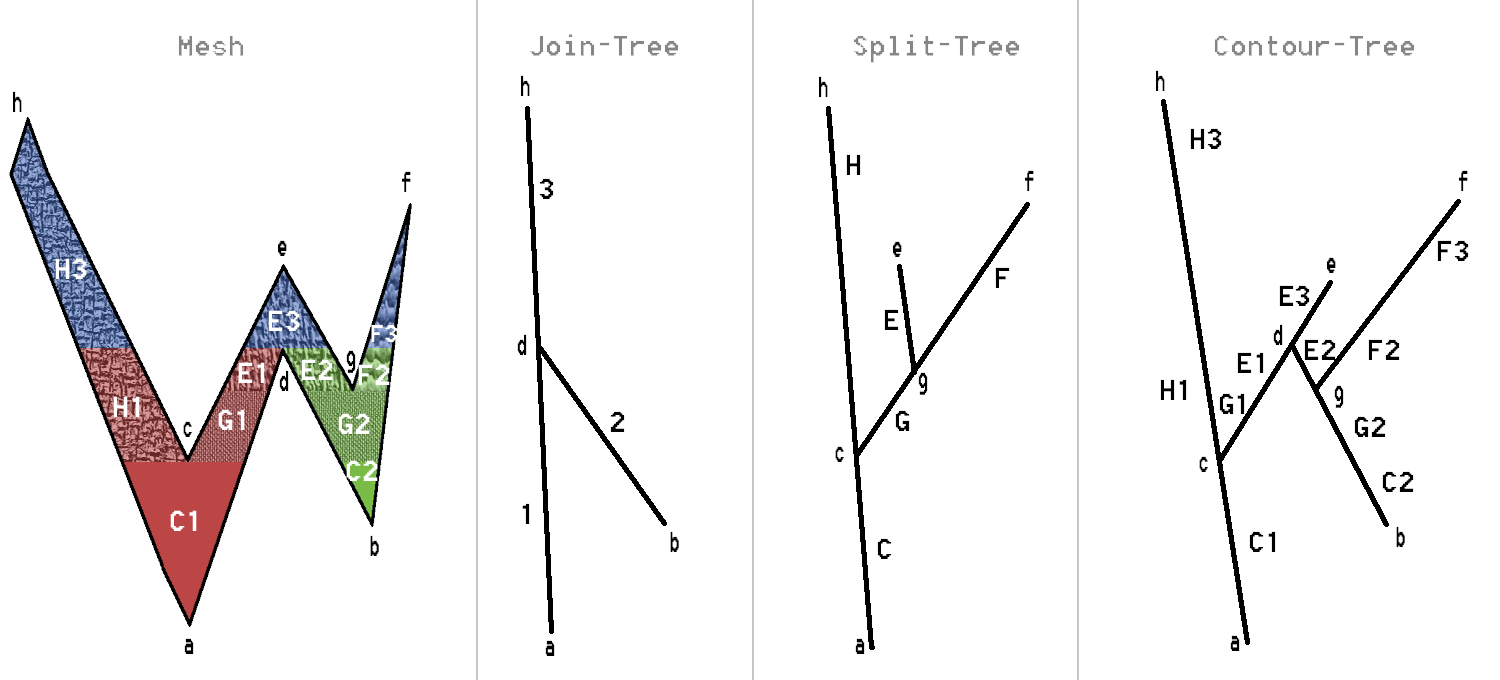
\includegraphics[width=\linewidth]{CounterExample.png}
    \caption{An encountered counter example. Considering first the arcs 1, 2 and 3 resulting in the join tree. Then consider the arc E: the arc 2 is split at g. The arc G now results in the split of arc 1 at c, but consequences of that split are not on the parent line of 1 (instead they are at g in arc 2)}
    \label{fig:ce}
\end{figure}

Because of this unsatisfactory break with the preceding task-parallel,  latency hiding, barrier free computation, an alternative strategy was explored. First consider the following observations:

An arc in the join/split tree represents a union of level set components in the data. If the split tree were to consist of only one arc, the arcs in the join tree would represent only a single level set component in the data and form the contour tree, and vice versa. Lets call the path of arcs leading from a starting arc upward to the global maximum (downward to the minimum for split trees) the parent line of the starting arc. The level set components represented by two arcs in the join/split tree that do not lie on each others parent lines are disjunct. That means, that all level set components represented by an arc in a tree only need to be separated by inner nodes of the other tree, until no arc represents multiple level set components. In other words inner nodes of the split tree split arcs of the join tree until the contour tree is reached, or vice versa. This is also the basis for the implicit construction of the contour tree, introduced in \cite{chiang}. There a contour tree arc is taken to be all those vertices in a certain join tree arc that also lie in a certain split tree arc and therefore form an isolated level set component. See figure 2 in \cite{chiang}.

These observations can be used to formulate an algorithm, similar to the implicit construction in \cite{chiang}, but explicitly and fitted to our distributed scenario.  Join and split arcs are reported to a master node in the cluster every time they are discovered. Starting with an empty tree this master node maintains a contour tree. For every new reported arc, the already known arcs are scanned, to check if the new arc subdivides them or is subdivided by them. This check needs the augmentation of arcs and therefore needs to send messages to all nodes involved with that arcs. If a subdivision takes place, all paths from the arc that was split need to be divided too. Some of the join/split events on the paths will belong to one of the subdivisions of the arc and some to the other, possibly creating two new paths. Once all arcs has been reported and handled in that way, the contour tree is finished. 

However there are multiple limitations to that approach. First polling the augmentation during execution will result in a lot of messages, that actually cause the progress to halt. Second while the arcs can be processed in any order, processing multiple at a time will require intensive use of synchronization. Third for every added arc the whole tree needs to be recalculated. This third aspect cannot be easily seen in the example provided by \cite{chiang}, where it seems, that an inner node will only ever divide one path from the arc it lies in, namely the parent line of that arc. However following this assumption the counter example in \ref{fig:ce} was encountered. Note that the implicit contour tree computed in \cite{chiang} of that counter example would include arcs that are subdivided unnecessarily or from another perspective multiple labels would point to parts of the same arc. This only comes to show, that the general approach of mutual subdivision of arcs from join and split tree, while being not sequential in nature, is a very global and intricate point of view. 

Considering these limitations and the produced overhead of this approach, collecting join and split tree in total on a central node and merge them partially in parallel as done in \cite{Carr} seems to be the best known approach.


\section{On the fly simplification and a possible metric with no prior knowledge}

When it comes to computing a contour tree, some kind of topological simplification is almost always necessary in reality. Our introduced approach is inherently good at simplifying the resulting join and split trees on the fly, that is without a global (or even local) barrier after construction and before simplification. The basic idea would be to calculate persistence of an arc right after the sweep terminates and the saddle is found. If the distance in function value between critical point and saddle of the arc is lower than a certain threshold, the arc is simply flagged disabled. The saddle still needs to inherit the boundary of the arc and vertices visited by the arc still need to count as visited for the saddle started arc. The augmentation post-processing in the end can simply move all vertices in disabled arcs upwards and override their function values with the value of the saddle (or whatever method for simplification is chosen). Flagged arcs will not be reported to the node responsible for join and split tree merging and will therefore not be found in the final contour tree.

While on the fly simplification is easy for a pre-defined persistence threshold another common input could be an approximately desired number of branches in the contour trees branch decomposition. Since we do not know which branch is gonna be more or less persistent or even how an average persistence may look like, on the fly simplification with a certain target number of branches is not trivial. However we can estimate an average persistence on the fly and base our simplification around it, by adapting the algorithm as follows:

Instead of interleaving minimum discovery and sweeping, we first discover all local minima and maxima in the data and broadcast the total number to all nodes. Only then we start with the sweeps. Keep track of the number of discovered terminated branches and their average persistence locally and exchange this information mutually between data chunks. With this we know the total number of branches, a sample size and empirical mean value. Estimating the distribution of branch persistences to be gaussian, we can therefore calculate a one sided (towards low persistence) confidence interval based on these numbers, setting the significance to the ratio of target branch number to discovered total branch count (equal to number of minima + maxima). This estimator will be very conservative at first, eliminating near to no branches, but with increasing sample size the confidence interval will become more narrow and start to eliminate outliers and will finally reach a size, where statistically the target number of branches should lie within the interval. 


\bibliographystyle{plain}
\bibliography{bib}


\end{document}                 % The input file ends with this command.

